%------------------------------------------------------------------------------
\chapter{Previous Work}
\label{ch:previous_work}

In order to display a realistic fire scene in a computer generated world, two procedures need to be performed.
Firstly, the fire dynamics have to be collected, this can either be done through a data capture session or simulated using fluid-based solvers.
Present techniques in the area are discussed below. 
Secondly, the gathered data will be visualized on the screen using some rendering method, a brief state-of-the-art review of fire rendering procedures is presented in Section~\ref{sec:rendering}.
We refer the interested readers to the more detailed survey on the topic, which has been recently presented by~\cite{Huang:2014}.

Fire simulation has received significantly more attention from the computer graphics community than fire rendering.
As the output data of the simulation methods is used in the rendering stage, an outline of the different simulation techniques is given below. 
Still, the main focus of this report lies in the rendering phase of the combustion simulation pipeline.

\section{Simulation}
\label{sec:simulation}

%\section{Fire Simulation}
%\label{sec:fire_simulation}

The techniques presented in this section are divided adopting the same criteria that was used by~\cite{Huang:2014}.
Since the categories are roughly chronological, the evolution of the field is easier to follow.

\textbf{Particle-based} methods were the first approach to simulate the visual animation of fire, as shown in Figures~\ref{fig:reeves_1983} and~\ref{fig:particle_based}.
A number of particles are emitted from certain locations, each particle has a set of attributes such as shape, velocity, color or lifetime.
The first model with particle systems was presented by~\cite{Reeves:1983}, the particles speed and colour were perturbed with a Gaussian noise at each time step, and the colour was subject to an additional linear perturbation on its lifetime.
Two particle systems were used in a hierarchy, one would control fire spread and the other a single explosion effect.
An extension was proposed by~\cite{Perry:1994}; the authors modified the particle system such that each particle shape would be defined by a series of non-overlapping coplanar triangles.
The transparency of each triangle increases towards the outer vertices, thus providing an improved visual effect.

\begin{figure}[htpb!]
        \centering
		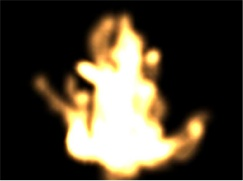
\includegraphics[width=0.4\textwidth]{img/perry_1994}
        \caption{Particle-based fire \cite{Perry:1994}.}
        \label{fig:particle_based}
\end{figure}

\textbf{Noise-based} methods focus on synthesizing the high fluctuation present in fire procedurally, as shown in Figure~\ref{fig:noise_based}.
The objective is to approximate the turbulence present in fire with an appropriate statistical model.
Using a variation of Perlin noise,~\cite{Perlin:1985} presented images of a corona of flames.
The method is limited to 2D, where the color is a combination of non-linear arbitrary functions.
This work was extended by~\cite{Perlin:1989} to 3D, where they used volumetric rendering to achieve improved results.
However, both methods have difficulties to handle interactions with other objects, and the variations in the synthesized images makes them incompatible for animation production. 

\begin{figure}[htpb!]
        \centering
        \begin{subfigure}[b]{0.45\textwidth}
                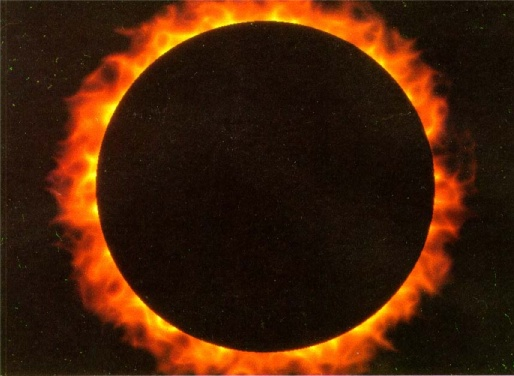
\includegraphics[width=\textwidth]{img/perlin_1985}
                \caption{\cite{Perlin:1985}.}
        \end{subfigure}%
        ~ %add desired spacing between images, e. g. ~, \quad, \qquad, \hfill etc.
          %(or a blank line to force the subfigure onto a new line)
        \begin{subfigure}[b]{0.45\textwidth}
                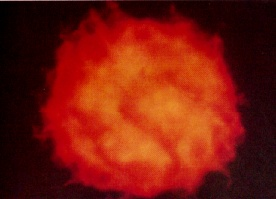
\includegraphics[width=\textwidth]{img/perlin_1989}
                \caption{\cite{Perlin:1989}.}
        \end{subfigure}  
        \caption{Noise-based fire examples.}
        \label{fig:noise_based}
\end{figure}

\textbf{Geometry skeleton} are driven by rendering primitives that represent the main features of fire, the high frequency details are built on top of the geometry structure, as shown in Figures~\ref{fig:lamorlette_2002} and~\ref{fig:geometry_skeleton}.
\cite{Lee:2001} presented a technique to animate fire on meshes, the flame front propagation is based on a geodesic flow field on the surface.
Although they achieved the effects of merging and separation of multiple flame fronts, the animators have no control over the evolution of the fire, as the only parameters are the initial fire conditions.
\cite{Lamorlette:2002} proposed a B-Spline curves interpolation method, details are added from a library of images which are then cast onto the profile of the flame.
The authors' technique supports a range of flame behaviour, such as spreading, flickering, and flame separation and merging.
In order to achieve real time simulations,~\cite{Bridault:2006} modelled the flame shape on NURBS surfaces on which a transparent 2D texture were mapped.

\begin{figure}[htpb!]
        \centering
        \begin{subfigure}[t]{0.41\textwidth}
                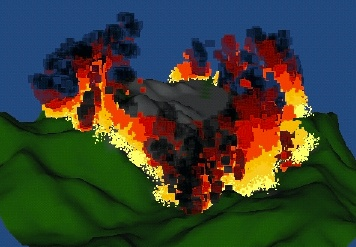
\includegraphics[width=\textwidth]{img/lee_2001}
                \caption{\cite{Lee:2001}.}
        \end{subfigure}%
        ~ %add desired spacing between images, e. g. ~, \quad, \qquad, \hfill etc.
          %(or a blank line to force the subfigure onto a new line)
        \begin{subfigure}[t]{0.36\textwidth}
                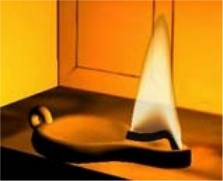
\includegraphics[width=\textwidth]{img/bridault_2006}
                \caption{\cite{Bridault:2006}.}
        \end{subfigure}          
        \caption{Geometry skeleton fire examples.}
        \label{fig:geometry_skeleton}
\end{figure}

\textbf{Data driven} methods are used to simulate fire with data from real flames, as shown in Figure~\ref{fig:data_driven}.
The quality of the animation depends directly on the data, and by avoiding the simulation stage the computational overhead is reduced significantly, as solving the underlying heat transport and other chemical equations is no longer needed.
However, there are severe limitations when producing new animations and interactions with other objects.
\cite{Rushmeier:1995} captured a heptane pool fire with water-cooled nitrogen-purged probes.
Using two images from orthographic camera views,~\cite{Hasinoff:2003} reconstructed 3D volumetric fire using tomographic techniques.
\cite{Ihrke:2004} extended the work by~\cite{Hasinoff:2003}, the authors presented a method to reconstruct fire volumes using trilinear basis functions in scenes recorded with eight cameras.
\cite{Zhang:2011} presented a method to synthesize new animation sequences based on previously simulated data.
A flow graph whose nodes connect resembling simulation states is built, similarity between nodes is measured based on flow pathline distances.
New frames with smooth transitions are created by traversing the graph through different paths.
\cite{Okabe:2015} proposed a reconstruction technique using a set of sparse images, that can also be applied to generate novel animations.
The authors approach is to define an optimization problem in terms of colour histograms and steerable coefficients, which they can use to retrieve an approximation of the appearance of the volume at new viewing angles.

\begin{figure}[htpb!]
        \centering
        \begin{subfigure}[t]{0.106\textwidth}
                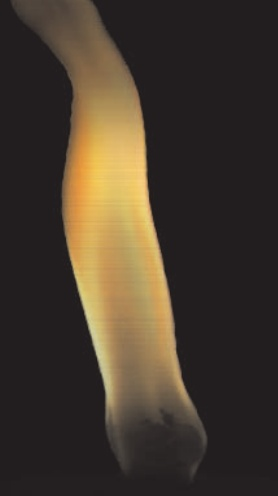
\includegraphics[width=\textwidth]{img/hasinoff_2003}
                \caption{\cite{Hasinoff:2003}.}
        \end{subfigure}  
        ~ %add desired spacing between images, e. g. ~, \quad, \qquad, \hfill etc.
          %(or a blank line to force the subfigure onto a new line)
        \begin{subfigure}[t]{0.19\textwidth}
                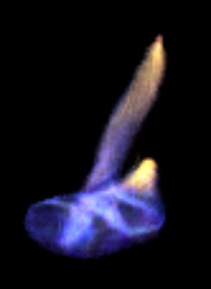
\includegraphics[width=\textwidth]{img/ihrke_2004}
                \caption{\cite{Ihrke:2004}.}
        \end{subfigure}      
        ~ %add desired spacing between images, e. g. ~, \quad, \qquad, \hfill etc.
          %(or a blank line to force the subfigure onto a new line)
        \begin{subfigure}[t]{0.29\textwidth}
                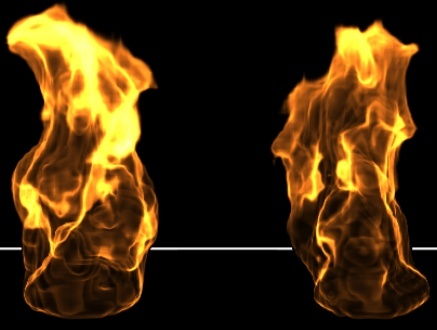
\includegraphics[width=\textwidth]{img/zhang_2011}
                \caption{\cite{Zhang:2011}.}
        \end{subfigure}     
        \begin{subfigure}[t]{0.33\textwidth}
                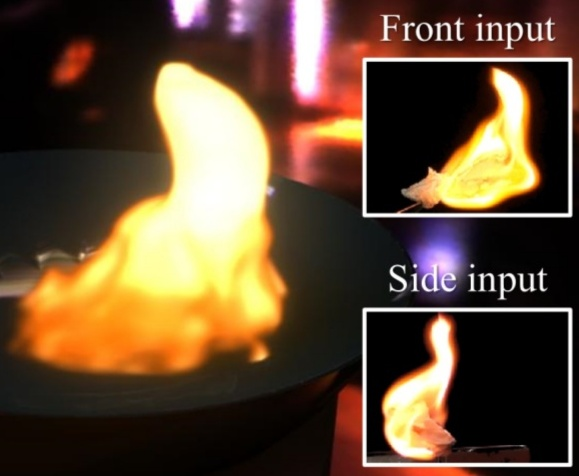
\includegraphics[width=\textwidth]{img/okabe_2015}
                \caption{\cite{Okabe:2015}.}
        \end{subfigure}%
        ~ %add desired spacing between images, e. g. ~, \quad, \qquad, \hfill etc.
          %(or a blank line to force the subfigure onto a new line)                      
        \caption{Date driven fire examples.}
        \label{fig:data_driven}
\end{figure}

\textbf{Physically-based} methods simulate the fire combustion processes, including flame propagation or the chemical reactions that convert fuel into gaseous products, as shown in Figures~\ref{fig:horvath_2009} and~\ref{fig:physically_based}.  
Incompressible flow equations were used by~\cite{Stam:1995} to drive a fire simulation.
Given initial fuel conditions, the fire spread is advected on a grid using an advection-diffusion type equation.
Building on a semi-Lagrangian fluid solver of~\cite{Stam:1999}, a model which includes gaseous fuel and gaseous byproducts was proposed by~\cite{Nguyen:2002}.
In order to include the characteristics of the noise-based methods, \cite{Hong:2007} combined the previous model with a set of third-order equations from detonation shock dynamics presented by~\cite{Yao:1996}.
As with the noise-based methods, this addition is visually attractive, yet it is not physically based. 
Capitalizing on the recent advances in GPUs parallel processing power, \cite{Horvath:2009} proposed a fixed camera model.
Particle properties are computed on a three-dimensional coarse grid, which are then projected into several view-dependant two-dimensional slices.
The authors' model is based on the assumption that fine variations, which are perpendicular to the projection plane, are not individually visible and, they do not significantly affect the overall flow.


\begin{figure}[htb!]
        \centering
        \begin{subfigure}[t]{0.2\textwidth}
                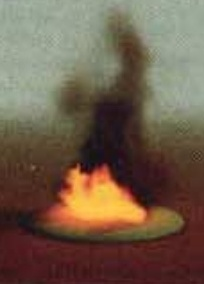
\includegraphics[width=\textwidth]{img/stam_1995}
                \caption{\cite{Stam:1995}.}
        \end{subfigure}%
        \quad %add desired spacing between images, e. g. ~, \quad, \qquad, \hfill etc.
          %(or a blank line to force the subfigure onto a new line)
        \begin{subfigure}[t]{0.22\textwidth}
                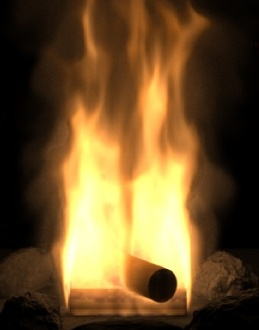
\includegraphics[width=\textwidth]{img/nguyen_2002}
                \caption{\cite{Nguyen:2002}.}
        \end{subfigure}       
        \quad %add desired spacing between images, e. g. ~, \quad, \qquad, \hfill etc.
          %(or a blank line to force the subfigure onto a new line)
        \begin{subfigure}[t]{0.3\textwidth}
                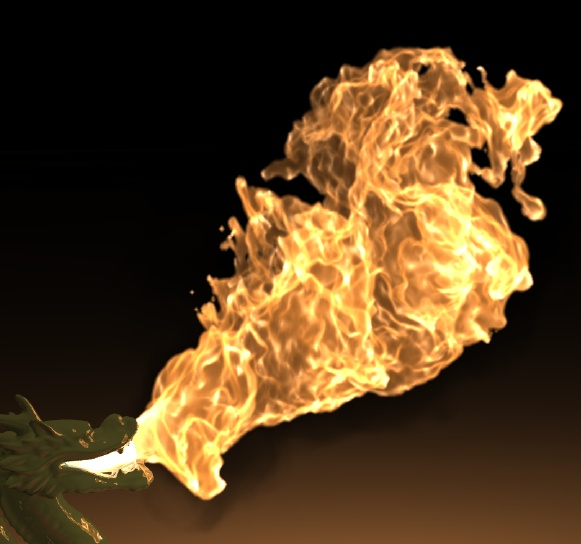
\includegraphics[width=\textwidth]{img/hong_2007}
                \caption{\cite{Hong:2007}.}
        \end{subfigure} 
        \caption{Physically-based fire examples.}
        \label{fig:physically_based}
\end{figure}
 
\textbf{Other effects} directly related to fire have also been explored, as shown in Figure~\ref{fig:other_effects}.
\cite{Feldman:2003} presented a model to simulate suspended particles during explosions.
An incompressible fluid model drives the motion of air and hot gases, and the suspended particles follow their movements.
\cite{Melek:2005} simulated the decomposition of an object as it undergoes combustion.
Heat is transferred between the different parts of the object and the air; the decomposition is modelled as a moving boundary spreading in the distance field of the object, where level set methods are used to compute the moving interfaces.
Credible sound is an important factor to increase the believability of a finished fire animation.
\cite{Chadwick:2011} proposed a method to automatically generate plausible noise given for a given fire simulation.
Low frequency sound is estimated using a physical model whose two given inputs are the flame front and heat release.
A data driven sound synthesis approach, based on the work by~\cite{Wei:2000}, is applied to generate the high frequency content.

\begin{figure}[htb!]
        \centering
        \begin{subfigure}[t]{0.175\textwidth}
                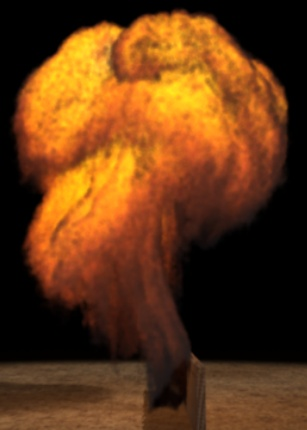
\includegraphics[width=\textwidth]{img/feldman_2003}
                \caption{\cite{Feldman:2003}.}
        \end{subfigure}%
        ~ %add desired spacing between images, e. g. ~, \quad, \qquad, \hfill etc.
          %(or a blank line to force the subfigure onto a new line)
        \begin{subfigure}[t]{0.4\textwidth}
                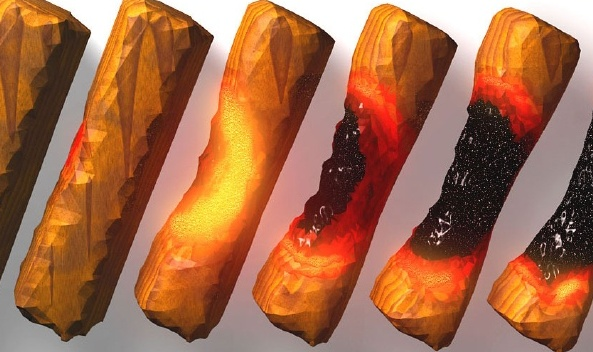
\includegraphics[width=\textwidth]{img/melek_2005}
                \caption{\cite{Melek:2005}.}
        \end{subfigure}  
        ~ %add desired spacing between images, e. g. ~, \quad, \qquad, \hfill etc.
          %(or a blank line to force the subfigure onto a new line)
        \begin{subfigure}[t]{0.3\textwidth}
                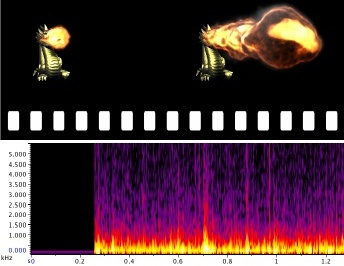
\includegraphics[width=\textwidth]{img/chadwick_2011}
                \caption{\cite{Chadwick:2011}.}
        \end{subfigure}          
        \caption{Other effects with fire.}
        \label{fig:other_effects}
\end{figure}

%\subsection{Smoke Simulation}
%\label{sec:smoke_simulation}


\section{Rendering}
\label{sec:rendering}

Rendering fire is more challenging than rendering other types of participating media, the main reason being that fire is a light-emitting source.
The luminescence radiated by a flame is generated by black body radiation due to the high temperature of the particles during the combustion process.
In order to realistically render fire, light absorption and scattering in the media, including air, has to be taken into consideration.
A succinct review of the current methods used by the computer graphics community for fire rendering is presented below.

\subsection{Raster-Based Methods}
\label{sec:raster_based}

Raster-based techniques sacrifice quality in the interest of interactive frame rates, renderings are shown in Figure~\ref{fig:raster_based}.
Generally, some form of texture mapping is applied, only the surface of the flame is considered, and the illumination of the scene is approximated using parameters which can be easily computed such as the fire height.

\cite{Reeves:1983} applied a linear colour assignment to each particle in their simulation based on their lifetime.
\cite{Lee:2001} applied the same technique to render fires on mesh surfaces, where a particle would begin with a light yellow colour, evolve to red and finish in black at the end of their lifetime.
\cite{Lamorlette:2002} presented a technique were a flame picture is mapped onto the two-dimensional flame profile with a base colour.
For each particle an intermediate emitting value is computed, and the final colour profile is super-sampled from an approximation of the cross-sectional area of the flame, as it would appear from the camera.
\cite{Westover:1990} introduced texture splats as a new rendering primitive, \cite{Wei:2002} rendered fire using Westover's technique.
Direct illumination is approximated by rendering the fire particles separately to create a light image, which is texture projected into the surrounding objects.
\cite{Zhao:2003} also proposed a method with flame particle splats, which are added with splats from other objects and sorted based on their distance to the screen plane.
The splats are projected in front-to-back order and alpha-blended to produce the end result.
\cite{Ihrke:2004} rendered fire realistically using a technique based on tomography reconstructions of real flames.
Precomputed ray-marching data is stored in a matrix, that is later used for fast reconstruction of new view points.
\cite{Bridault:2006} used a spectrophotometer to capture photometric distributions of candles.
The intensities are stored on a texture and changes in illumination over time are introduced with an attenuation factor which is proportional to the size of the flame.
\cite{Zhang:2011} proposed a method were fire particles and their attributes are first projected onto a set of slicing planes, which are orthogonal to the camera direction. 
The planes are then blended in back-to-front order, and a one-dimensional colour texture is used as a transfer function to convert flow attributes to colours and opacities. 
\cite{Jamriska:2015} recently proposed a texture synthesis method to generate fire animations.
The method requires a hand made motion field and an alpha mask of the desired result, both are used to generate the new sequence using data from an existing video exemplar.

\begin{figure}[htpb!]
        \centering
       \begin{subfigure}[t]{0.3\textwidth}
                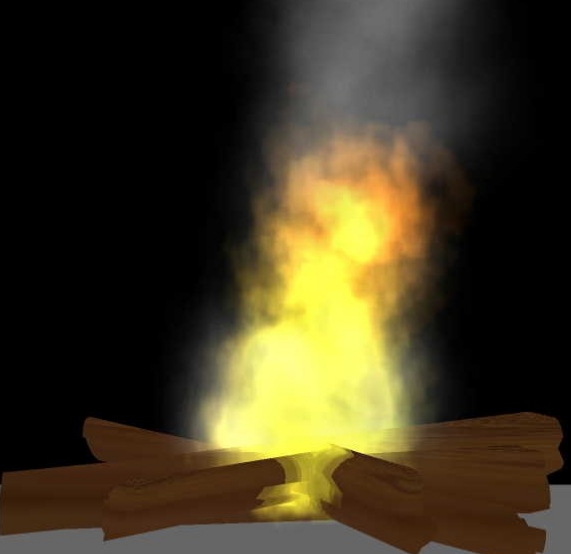
\includegraphics[width=\textwidth]{img/wei_2002}
                \caption{\cite{Wei:2002}.}
        \end{subfigure}%
        ~        
        \begin{subfigure}[t]{0.285\textwidth}
                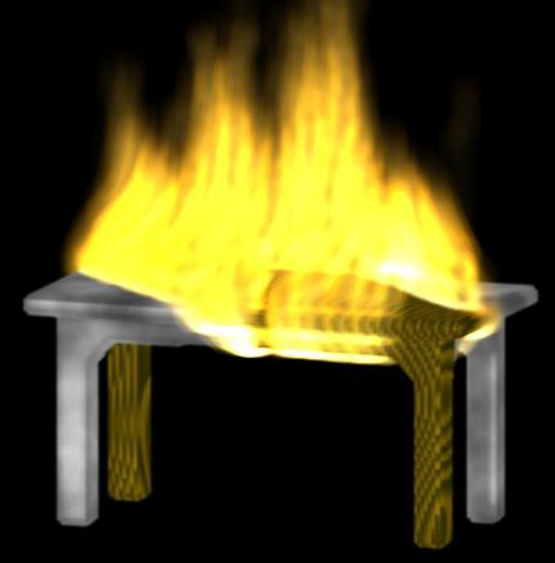
\includegraphics[width=\textwidth]{img/zhao_2003}
                \caption{\cite{Zhao:2003}.}
        \end{subfigure}% 
		~        
        \begin{subfigure}[t]{0.36\textwidth}
                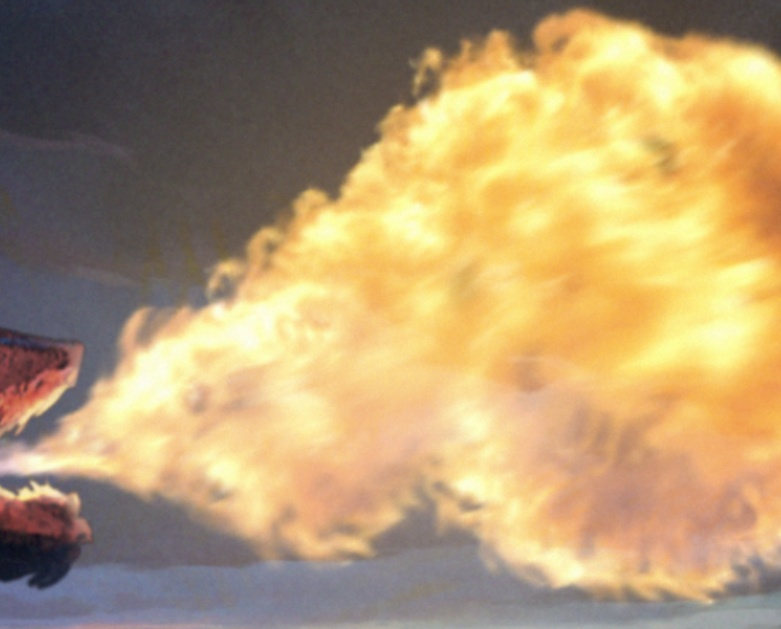
\includegraphics[width=\textwidth]{img/jamriska_2015}
                \caption{\cite{Jamriska:2015}.}
        \end{subfigure}%         
        \caption{Raster-based techniques.}
        \label{fig:raster_based}
\end{figure}



\subsection{Ray-Tracing-Based Methods}
\label{sec:ray_tracing_based}

Volume ray-tracing techniques offer astonishing results, however the associated computational costs are considerable.
Rays are shot from the view plane and evaluated at small increments; the total radiance at the origin of the ray is computed by integrating the radiance at each step.
A further drawback of ray tracing techniques, in comparison to raster-based methods, is the lack of a standard ray-tracing pipeline.

\cite{Rushmeier:1995} presented a method to perform accurate ray casting on sparse measured data.
The fire was modelled as a series of stacked cylindrical rings, where each ring has uniform properties.
The total radiance at each point is integrated using a Monte Carlo method, summing up the measured irradiances at sample locations. 
\cite{Nguyen:2002} proposed a ray marching technique to solve the Radiative Transport Equation, see Chapter~\ref{ch:methodology}.
The emitted light is computed using Planck's formula of black body radiation, scattering in the media and visual adaptation to the fire spectra are modelled.
\cite{Feldman:2003} also included black body radiation in their animation of fire with suspended particles, however the mapping to RGB was manually adjusted to match the images of real explosions.
Direct illumination shadows were computed using deep shadow maps~\cite{Lokovic:2000}, while scattering and illumination by other objects in the scene used the technique proposed by~\cite{Jensen:2002}.
An extension to~\cite{Nguyen:2002} was presented by~\cite{Pegoraro:2006}, the authors' model has physically-based absorption, emission and scattering properties.
The spectroscopy characteristics of different fuels are achieved by modelling the transitions of electrons between different states in the molecules.
Non-linear trajectories of light in the medium due to light refraction effects are included as well.
In order to minimize the effects induced by the limitations of the RGB colour space, the visual adaptation process is presented as a post-processing effect.
\cite{Horvath:2009} proposed a rendering method whose main objective was user-friendliness for artists.
Using the fixed camera slices described in Section~\ref{sec:simulation}, the authors perform simple volume rendering to join them in a single image.
Black body radiation is used for the light, the images are motion-blurred with a filter based on the velocities in the slices, and the heat distortion is added as post-processing filter defined by the user. 